% Figure s03f06_helical (Session 3): schematic edge dispersions, chiral against helical.
% The image is rendered by figures/blender/s03f06_helical.py; the coordinates of the labels come from
% figures/blender/out/s03f06_helical_anchors.tex. Build with figures/blender/build_figure.sh s03f06_helical.
\documentclass[11pt,tikz,border=0pt]{standalone}
\usepackage[T1]{fontenc}
\usepackage{amsmath,amssymb,graphicx,bm}
\usepackage{xcolor}
\usetikzlibrary{arrows.meta,calc}
% The three label colors of the figures, with the same values as in src/figures_preamble.tex.
\definecolor{aqmaccent}{RGB}{31,78,121}
\definecolor{aqmbroken}{RGB}{168,42,34}
\definecolor{aqmmuted}{RGB}{125,125,125}

\newlength{\figw}\setlength{\figw}{15.6cm}   % the text width of the notes (A4, 2.7 cm margins)

\begin{document}
\begin{tikzpicture}[lbl/.style={font=\small, inner sep=1.5pt}, pnl/.style={font=\small\bfseries, inner sep=1.5pt}]
  \node[anchor=south west, inner sep=0pt] at (0,0)
    {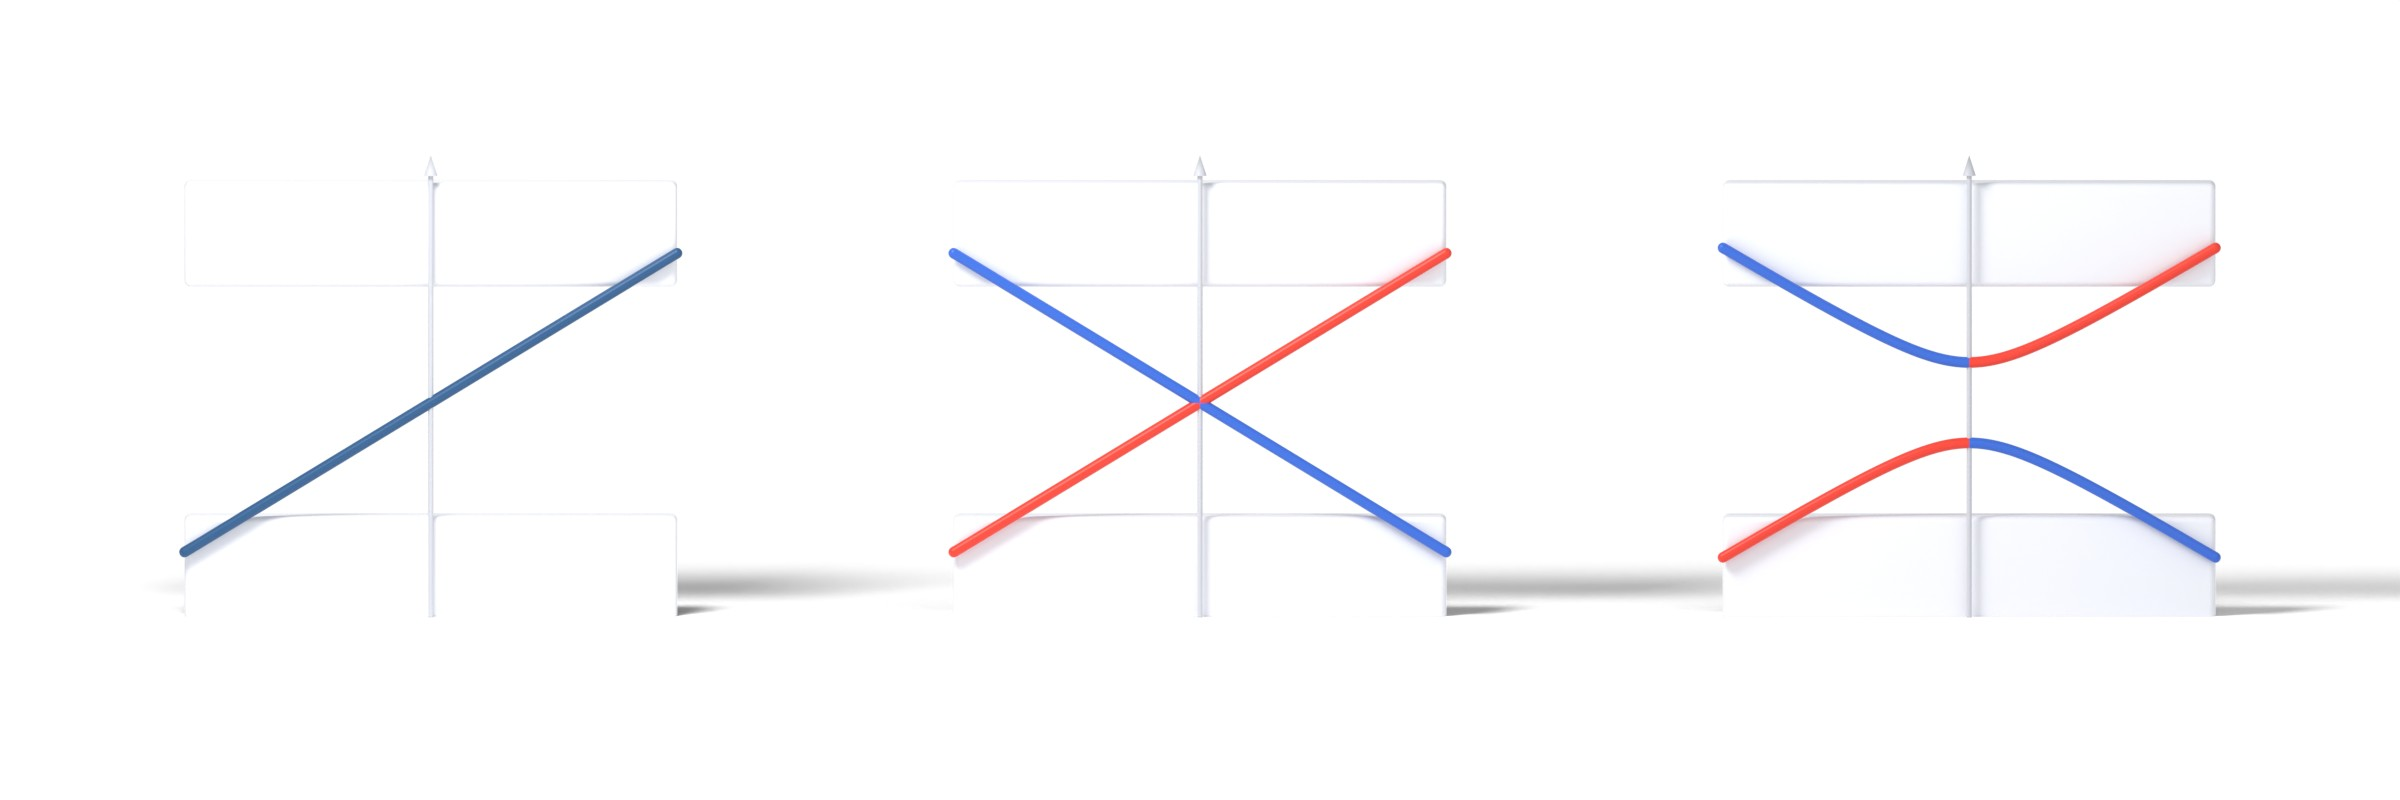
\includegraphics[width=\figw]{../blender/out/s03f06_helical.jpg}};
  %% written by figlib.py; x and y in units of the image width
\coordinate (aE) at (0.1795\figw,0.2685\figw);
\coordinate (ak) at (0.3013\figw,0.0674\figw);
\coordinate (atitle) at (0.0769\figw,0.2685\figw);
\coordinate (abelow) at (0.1795\figw,0.0650\figw);
\coordinate (abulk) at (0.2821\figw,0.2350\figw);
\coordinate (bE) at (0.5000\figw,0.2685\figw);
\coordinate (bk) at (0.6218\figw,0.0674\figw);
\coordinate (btitle) at (0.3974\figw,0.2685\figw);
\coordinate (bbelow) at (0.5000\figw,0.0650\figw);
\coordinate (bbulk) at (0.6026\figw,0.2350\figw);
\coordinate (cDelta) at (0.8245\figw,0.1655\figw);
\coordinate (cE) at (0.8205\figw,0.2685\figw);
\coordinate (ck) at (0.9423\figw,0.0674\figw);
\coordinate (ctitle) at (0.7179\figw,0.2685\figw);
\coordinate (cbelow) at (0.8205\figw,0.0650\figw);
\coordinate (cbulk) at (0.9231\figw,0.2350\figw);

  \node[lbl, anchor=south west] at (atitle) {\textbf{(a)}\quad chiral};
  \node[lbl, anchor=south west] at (btitle) {\textbf{(b)}\quad helical};
  \node[lbl, anchor=south west] at (ctitle) {\textbf{(c)}\quad time reversal broken};
  \foreach \p in {a,b,c} {
    \node[lbl, anchor=south east] at (\p k) {$k$};
    \node[lbl, anchor=west, text=aqmmuted] at (\p bulk) {bulk};
  }
  \node[lbl, anchor=west, text=aqmbroken] at (cDelta) {$2\Delta$};
\end{tikzpicture}
\end{document}
